
\documentclass{beamer}
%\documentclass[handout]{beamer}

% THEME SETTINGS %%%%%%%%%%%%
\usetheme[secheader]{Boadilla}
\usecolortheme{default}
\useinnertheme{circles}
\setbeamertemplate{blocks}[default]

% Get rid of bottom navigation bars
\setbeamertemplate{footline}[page number]{}

% Gets rid of navigation symbols
\setbeamertemplate{navigation symbols}{}

% PACKAGES %%%%%%%%%%%%%%%%%%%
\usepackage{listings}
\usepackage{xcolor}
\usepackage{multirow}
\usepackage{array}
\usepackage{verbatim}
\usepackage{pbox}

% LISTINGS STYLE %%%%%%%%%%%%%
\definecolor{bluekeywords}{rgb}{0.13,0.13,1}
\definecolor{greencomments}{rgb}{0,0.5,0}
\definecolor{redstrings}{rgb}{0.9,0,0}
\definecolor{listingsbg}{HTML}{EFEFFF}

\lstset{language=C++,
  showspaces=false,            % show spaces adding particular underscores
  showtabs=false,              % show tabs within strings adding particular underscores
  breaklines=true,             % sets automatic line breaking
  showstringspaces=false,      % underline spaces within strings
  breakatwhitespace=true,      % sets if automatic breaks should only happen at whitespace
  captionpos=b,                % sets the caption-position to bottom
  escapeinside={(*@}{@*)},
  commentstyle=\color{greencomments},
  keywordstyle=\color{bluekeywords}\bfseries,
  stringstyle=\color{redstrings},
  basicstyle=\ttfamily\fontsize{9}{10}\selectfont,
  backgroundcolor=\color{listingsbg},
}

% MACROS %%%%%%%%%%%%%%%%%%%%%
\newcommand{\lstsrctitle}[0]{%
 {\scriptsize\lstname}
}

\newcommand{\kw}[1]{\texttt{\textcolor{bluekeywords}{\ttfamily\fontsize{9}{10}\selectfont #1}}}

\newenvironment{varblock}[3]{%
  \setbeamercolor{block body}{#2}
  \setbeamercolor{block title}{#3}
  \begin{block}{#1}}{\end{block}}

% Colours taken from http://twitter.github.com/bootstrap/components.html#alerts
% Do block %%%%%%%%%%%%%%%%%%%%%%
\definecolor{doblocktext}{HTML}{468847}
\definecolor{doblockbg}{HTML}{DFF0D8}
\newenvironment{doblocke}[1]{% begin
  \begin{varblock}{\textbf{Do}}%
  {bg=doblockbg,fg=doblocktext}{bg=doblocktext,fg=white}%
  \lstset{backgroundcolor=}% The background should be the same as that of the block
  #1}%
  {\end{varblock}} %end
\newcommand{\doblock}[1]{%
 \begin{doblocke}#1\end{doblocke} 
}

% Don't block %%%%%%%%%%%%%%%%%%%
\definecolor{dontblocktext}{HTML}{B94A48}
\definecolor{dontblockbg}{HTML}{F2DEDE}  
\newenvironment{dontblocke}[1]{% begin
  \begin{varblock}{\textbf{Don't}}%
  {bg=dontblockbg,fg=dontblocktext}{bg=dontblocktext,fg=white}
  \lstset{backgroundcolor=}% The background should be the same as that of the block
  #1}%
  {\end{varblock}} %end

\newcommand{\dontblock}[1]{%
 \begin{varblock}{\textbf{Don't}}{bg=dontblockbg,fg=dontblocktext}{bg=dontblockbg,fg=dontblocktext}
 #1
 \end{varblock} 
}

\definecolor{defiblocktext}{HTML}{3A87AD}
\definecolor{defiblockbg}{HTML}{D9EDF7}
\newcommand{\defiblock}[2]{%
 \begin{varblock}{\textbf{Definition}}%
 {bg=defiblockbg,fg=defiblocktext}{bg=defiblocktext,fg=white}
  \begin{tabular}{ll}\textit{#1} & #2\end{tabular}
 \end{varblock} 
}

\definecolor{warnblocktext}{HTML}{C09853}
\definecolor{warnblockbg}{HTML}{D9EDF7}
\newcommand{\warnblock}[1]{%
 \begin{varblock}{\textbf{Warning!}}{bg=warnblockbg,fg=warnblocktext}{bg=warnblockbg,fg=warnblocktext}
  #1
 \end{varblock} 
}

\newcommand{\cout}[1]{%
 Output: \pbox[t]{\textwidth}{\ttfamily\fontsize{9}{10}\selectfont{}#1}
}

\title{Scientific C++}
\subtitle{An introduction}
\author{Martin Uhrin}
\institute{UCL}
\date{November 7-9th 2012}

\begin{document}

\frame{\titlepage}

\begin{frame}
\frametitle{Table of Contents}
\tableofcontents
\end{frame}

\documentclass{beamer}
%\documentclass[handout]{beamer}

% Input all common stuff


% THEME SETTINGS %%%%%%%%%%%%
\usetheme[secheader]{Boadilla}
\usecolortheme{default}
\useinnertheme{circles}
\setbeamertemplate{blocks}[default]

% Get rid of bottom navigation bars
\setbeamertemplate{footline}[page number]{}

% Gets rid of navigation symbols
\setbeamertemplate{navigation symbols}{}

% PACKAGES %%%%%%%%%%%%%%%%%%%
\usepackage{listings}
\usepackage{xcolor}
\usepackage{multirow}
\usepackage{array}
\usepackage{verbatim}
\usepackage{pbox}
\usepackage{tabularx}

% LISTINGS STYLE %%%%%%%%%%%%%
\definecolor{bluekeywords}{rgb}{0.13,0.13,1}
\definecolor{greencomments}{rgb}{0,0.5,0}
\definecolor{redstrings}{rgb}{0.9,0,0}
\definecolor{listingsbg}{HTML}{EFEFFF}

\lstset{language=C++,
  showspaces=false,            % show spaces adding particular underscores
  showtabs=false,              % show tabs within strings adding particular underscores
  breaklines=true,             % sets automatic line breaking
  showstringspaces=false,      % underline spaces within strings
  breakatwhitespace=true,      % sets if automatic breaks should only happen at whitespace
  captionpos=b,                % sets the caption-position to bottom
  escapeinside={(*@}{@*)},
  commentstyle=\color{greencomments},
  keywordstyle=\color{bluekeywords}\bfseries,
  stringstyle=\color{redstrings},
  basicstyle=\ttfamily\fontsize{9}{10}\selectfont,
  backgroundcolor=\color{listingsbg}
}

% MACROS %%%%%%%%%%%%%%%%%%%%%
\newcommand{\lstsrctitle}[0]{%
 {\scriptsize\lstname}
}

\newcommand{\kw}[1]{\texttt{\textcolor{bluekeywords}{\ttfamily\fontsize{9}{10}\selectfont #1}}}

\newenvironment{varblock}[3]{%
  \setbeamercolor{block body}{#2}
  \setbeamercolor{block title}{#3}
  \begin{block}{#1}}{\end{block}}

% Colours taken from http://twitter.github.com/bootstrap/components.html#alerts
% Do block %%%%%%%%%%%%%%%%%%%%%%
\definecolor{doblocktext}{HTML}{468847}
\definecolor{doblockbg}{HTML}{DFF0D8}
\newenvironment{doblocke}[0]{% begin
  \begin{varblock}{\textbf{Do}}%
  {bg=doblockbg,fg=doblocktext}{bg=doblocktext,fg=white}%
  \setbeamercolor{itemize item}{fg=doblocktext}
  \lstset{backgroundcolor=}% The background should be the same as that of the block
  } % begin
  {\end{varblock}} %end
  
\newcommand{\doblock}[1]{%
 \begin{doblocke}#1\end{doblocke} 
}

% Don't block %%%%%%%%%%%%%%%%%%%
\definecolor{dontblocktext}{HTML}{B94A48}
\definecolor{dontblockbg}{HTML}{F2DEDE}  
\newenvironment{dontblocke}[0]{% begin
  \begin{varblock}{\textbf{Don't}}%
  {bg=dontblockbg,fg=dontblocktext}{bg=dontblocktext,fg=white}
  \setbeamercolor{itemize item}{fg=dontblocktext}
  \lstset{backgroundcolor=}% The background should be the same as that of the block
  }%
  {\end{varblock}} %end

\newcommand{\dontblock}[1]{%
 \begin{dontblocke}#1\end{dontblocke} 
}

% Defi block %%%%%%%%%%%%%%%%%%%%
\definecolor{defiblocktext}{HTML}{3A87AD}
\definecolor{defiblockbg}{HTML}{D9EDF7}
\newenvironment{defiblocke}[1]{% begin
  \begin{varblock}{\textbf{Definition}}%
  {bg=defiblockbg,fg=defiblocktext}{bg=defiblocktext,fg=white}
  \lstset{backgroundcolor=}% The background should be the same as that of the block
  \textit{#1} }
  {\end{varblock}} %end

\newcommand{\defiblock}[2]{%
 \begin{varblock}{\textbf{Definition}}%
 {bg=defiblockbg,fg=defiblocktext}{bg=defiblocktext,fg=white}%
  \begin{tabularx}{\linewidth}{lX}\textit{#1} & #2\end{tabularx}
 \end{varblock} 
}

\newenvironment{defiblockbaree}[1]{ %begin
  \begin{varblock}{\textbf{#1}}%
  {bg=defiblockbg,fg=defiblocktext}{bg=defiblocktext,fg=white}
  \lstset{backgroundcolor=}} %begin
  {\end{varblock}} %end

\definecolor{warnblocktext}{HTML}{C09853}
\definecolor{warnblockbg}{HTML}{FCF8E3}
\newenvironment{warnblocke}[0]{% begin
  \begin{varblock}{\textbf{Warning!}}%
  {bg=warnblockbg,fg=warnblocktext}{bg=warnblocktext,fg=white}
  \lstset{backgroundcolor=}% The background should be the same as that of the block
  \setbeamercolor{itemize item}{fg=warnblocktext}
  \setbeamercolor{item projected}{fg=white,bg=warnblocktext}
  } % begin
  {\end{varblock}} % end

\newcommand{\warnblock}[1]{%
  \begin{warnblocke}#1\end{warnblocke}
} % newcommand

\newcommand{\cout}[1]{%
 Output: \pbox[t]{\textwidth}{\ttfamily\fontsize{9}{10}\selectfont{}#1}
}

\newenvironment{doitemize}[0]{%
  \begin{itemize}}%
  {\end{itemize}} %end


% CONSTANTS %%%%%%%%%%%%%%%%%%%%%%%%%%%

%Symbol for backslash in texttt \char`\\

% Common title slide stuff
\title{Introduction to Scientific Programming with C++}
\author{Martin Uhrin}
\institute{UCL}
\date{February 11-13th 2013}

\subtitle{Session 0: Basics}

\usepackage{graphicx}

\begin{document}

\frame{\titlepage}

\begin{frame}
\frametitle{Table of Contents}
\tableofcontents
\end{frame}

\section{Introduction to language}

\begin{frame}
	\frametitle{Introduction to C++}
	\framesubtitle{A little history}
	\begin{itemize}
	  \item<1->{Created in 1979 as an extension of C by this guy:\pause
		\begin{figure}
			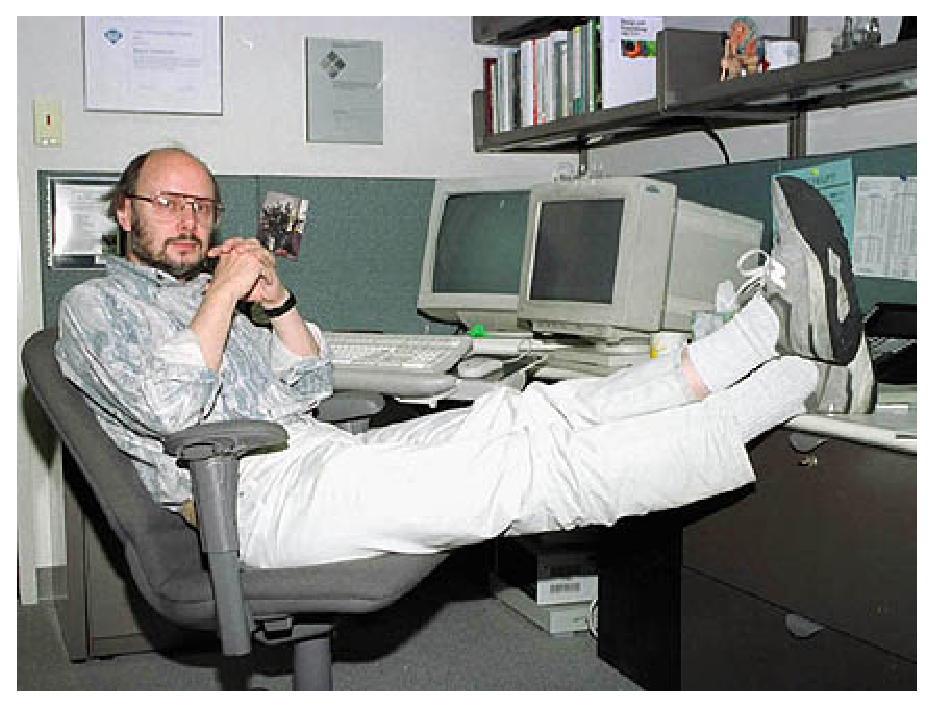
\includegraphics[height=30mm]{./figs/BjarneStroustrup.eps}
			\caption{Bjarne Stroustrup, creator of C++.}
		\end{figure}}
	  \item<3->{Built to be fast \textit{and} scalable and so has a mix of high and low-level constructs.}
	\end{itemize}
	
\end{frame}


\section{Program structure}

%Perhaps the best way to learn a programming language is to dive in and see what it's all about with a simple example.

%Here's out first program:

\begin{frame}[fragile]
  \frametitle{Hello World!}
  \framesubtitle{Where it all begins}

  \begin{columns}[t]
    \begin{column}[T]{0.55\textwidth}	\lstinputlisting[language=C++,title=\lstsrctitle,aboveskip=0pt]{../code/0_basics/lectures/hello_world.cpp}
    \end{column}
    \begin{column}[T]{0.45\textwidth}
			\cout{Hello world!}
		\end{column}
	\end{columns}
\end{frame}


\begin{frame}[fragile]
  \frametitle{Hello World dissection}
  \begin{semiverbatim}
  \uncover<1->{// My first C++ program
  }
  \uncover<2->{#include <iostream>
  }
  \uncover<3->{int main()}
  \uncover<4->{\{}
  \uncover<6->{  std::}\uncover<5->{cout << "Hello World!";}
  \uncover<7->{  return 0;}
  \uncover<4->{\}}
  \end{semiverbatim}
\end{frame}

\begin{frame}
  \frametitle{Going from source code to an executable}
  
  \begin{figure}%
    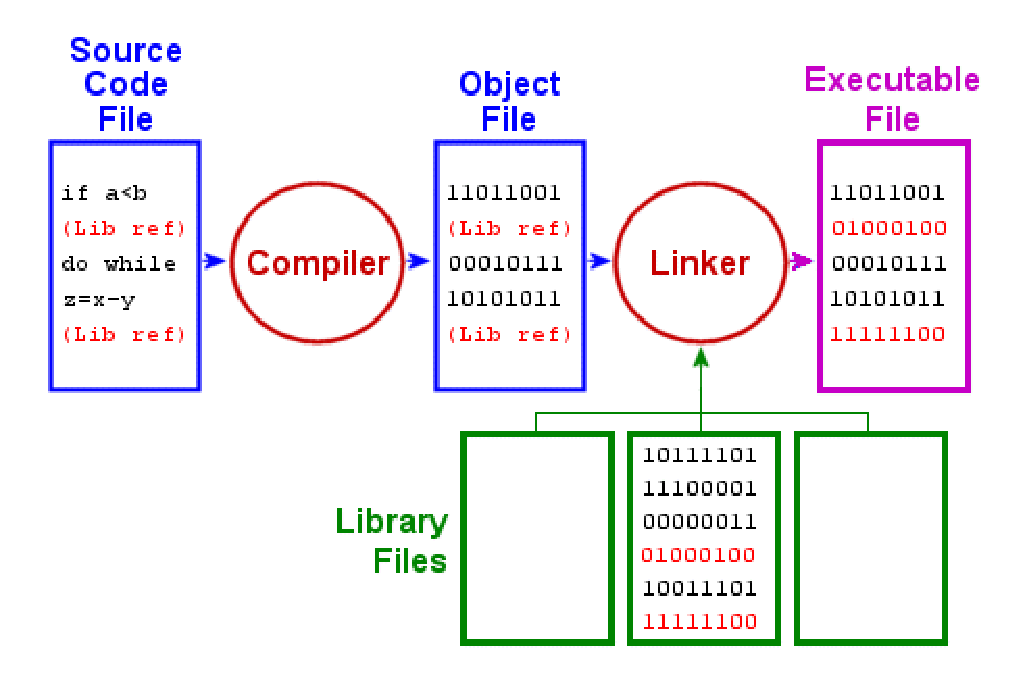
\includegraphics[width=0.6\columnwidth]{figs/compile.eps}%
    \caption{Compilation and linking of a C++ program\footnote{Source \url{http://www.aboutdebian.com/compile.htm} \copyright{} Keith Parkansky}.}%
  \end{figure}
  \pause There are range of compilers, some common ones are \emph{g++} (GNU), \emph{icc} (Intel), \emph{pgicc} (PGI) and others. 

\end{frame}

\begin{frame}[fragile]
  \frametitle{Whitespace}
  \defiblock{whitespace}{spaces, tabs, and (sometimes) new lines.}
  \pause
  
  Completely equivalent as far as compiler is concerned:
  \begin{lstlisting}
#include <iostream>
int main(){std::cout<<"Hello world!";return 0;}
  \end{lstlisting}
  \begin{lstlisting}
#include <iostream>
int main()
{
std::cout
<<
"Hello world!"
;
return
0
;
}  \end{lstlisting}
\end{frame}

\begin{frame}[fragile]
  \frametitle{Case sensitivity}
  C++ is case sensitive!  This means that:
  \begin{lstlisting}
int main()
  \end{lstlisting}
  is different from
  \begin{lstlisting}
INT MAIN ()
  \end{lstlisting}
  which is different from
  \begin{lstlisting}
int Main()
  \end{lstlisting}
  and only the first version is correct.
\end{frame}

\begin{frame}[fragile]
  \frametitle{Comments}
  Two types of comment can be used:
  \begin{lstlisting}
// This is a line comment.
// It ends at the end of the line.
// int myVariable = 0; This code will not execute!
  \end{lstlisting}
  \begin{lstlisting}
/* This is a C-style comment.
   It ends when the closing star-slash is reached. */
  \end{lstlisting}
    Use comments liberally - they are enormously useful!
    \doblock{Avoid stating the obvious.  A good comment will not say \textit{what} is happening but rather \textit{why}.}
\end{frame}

\section{Variables, constants and data types}

\subsection{Defining variables}

\begin{frame}[fragile]
\frametitle{Defining a variable}
  \defiblock{variable}{A named portion of memory used to store a determined value.}
  Let's define some variables:
  \begin{lstlisting}
int anInteger;
double aDouble;
unsigned short i;
float x, y, z;
  \end{lstlisting}
Format: \texttt{\textcolor{bluekeywords}{variable\_type} variable\_name, variable\_name2;}

\end{frame}

\subsection{Naming variables}

\begin{frame}
  \frametitle{Naming variables}
  
  A variable name is an example of an identifier.
  \defiblock{identifier}{an identifier is a sequence of characters used to denote the name of a variable, function\footnote{We'll see what these are shortly.}, class\footnotemark[\value{footnote}] or any entity you need to refer to in your code.}
  \pause
  Identifiers can be any sequence of letters, digits or underscore characters but they must \emph{not}:
	\begin{itemize}
  	\item start with a digit,
	  \item be one of the reserved keywords\footnote{See \url{http://en.cppreference.com/w/cpp/keyword} for full list.}.
	\end{itemize}
	\pause
	\defiblock{keyword}{a word that has a special meaning in the C++ language.}
\end{frame}

\begin{frame}[fragile]
  \frametitle{Naming variables}
  \begin{doblocke}
    \begin{doitemize}
      \item{
			Give variables meaningful names, even if this means more typing!\newline
			Good: \texttt{daysOfWeek, sumSq, isEnabled, unitCell}\newline
			Would the variable name make sense in that context when looking at the code a year later?
			}
			\pause
		  \item{Use variable names, much like comment, to convey intent, e.g.:
		  \begin{lstlisting}
		  double rootMeanSquare; // .. go on to calculate rms
		  \end{lstlisting}}
		  This will make it obvious to the user that the code after this variable should calculate the rms and store it in this variable.
		\end{doitemize}
	\end{doblocke}
	\pause
	\begin{dontblocke}
	  Use abbreviations unless they're VERY common.\newline
	  Use bad names: \texttt{data, dRange, a, ccn, value, one}
	\end{dontblocke}
\end{frame}

\begin{frame}[fragile]
  \frametitle{Variable types}
  Fundamental data types:

% Make the table less cramped vertically. 
% Make sure to reset to 1 after the table!
\renewcommand{\arraystretch}{1.1}
\begin{tabular}{lll}
\hline
Type & Size & Values \\
\hline
\kw{bool} & 1 byte & true or false \\
\kw{int} & 4 bytes & -2,147,483,648 to 2,147,483,647 \\
\kw{double} & 8 bytes & 2.2e-308 to 1.8e308\\ \pause
\kw{char} & 1 byte & 256 character values \\
\kw{unsigned short int} & 2 bytes & 0 to 65,353 \\
\kw{short int} & 2 bytes & -32,768 to 32,767 \\
\kw{unsigned int} & 4 bytes & 0 to 4,294,967,295 \\
\kw{unsigned long int} & 8 bytes & 0 to 18,446,744,073,709,551,615 \\
\kw{long int} & 8 bytes & -9,223,372,036,854,775,807 to \\
 & & 9,223,372,036,854,775,807 \\
\kw{float} & 4 bytes & 1.2e-38 to 3.4e38 
\end{tabular}
\end{frame}
\renewcommand{\arraystretch}{1}

\begin{frame}[fragile]
 \frametitle{Using variables}
 \lstinputlisting[language=C++,title=\lstsrctitle]{../code/0_basics/lectures/force_calc.cpp}
 Pretty easy, right?
\end{frame}

\subsection{Constants}

\begin{frame}[fragile]
\frametitle{Constants}
Spot the difference:
 \lstinputlisting[language=C++,basicstyle=\ttfamily\fontsize{6}{7}\selectfont,title=\lstsrctitle]{../code/0_basics/lectures/force_calc_const.cpp}
 \pause
 \doblock{Make everything \kw{const} unless it absolutely has to vary.  This has benefits for both the speed and correctness of your code.}
\end{frame}

\subsection{Scope}

\begin{frame}[fragile]
  \frametitle{Scope}
  \framesubtitle{All variables have a finite life time. They are created and \emph{destroyed}!}
  
  \begin{columns}[t]
    \begin{column}[T]{0.52\textwidth}
  		\defiblock{scope}{the region of a program that a variable can be used in.  This determines the ``lifetime'' of a variable.}
  		The scope of a variable is defined by the block, formed by braces \texttt{\{\}}, within which it is declared.
    \end{column}
    \pause
    \begin{column}[T]{0.42\textwidth}    
			\vspace*{-0.3cm} % I give up, aligning this properly is an arse!
			\begin{figure}[!ht]
			  \setlength{\textfloatsep}{0pt}
			  \setlength{\floatsep}{0pt}
				\setlength{\abovecaptionskip}{0pt}
			  \setlength{\belowcaptionskip}{0pt}
				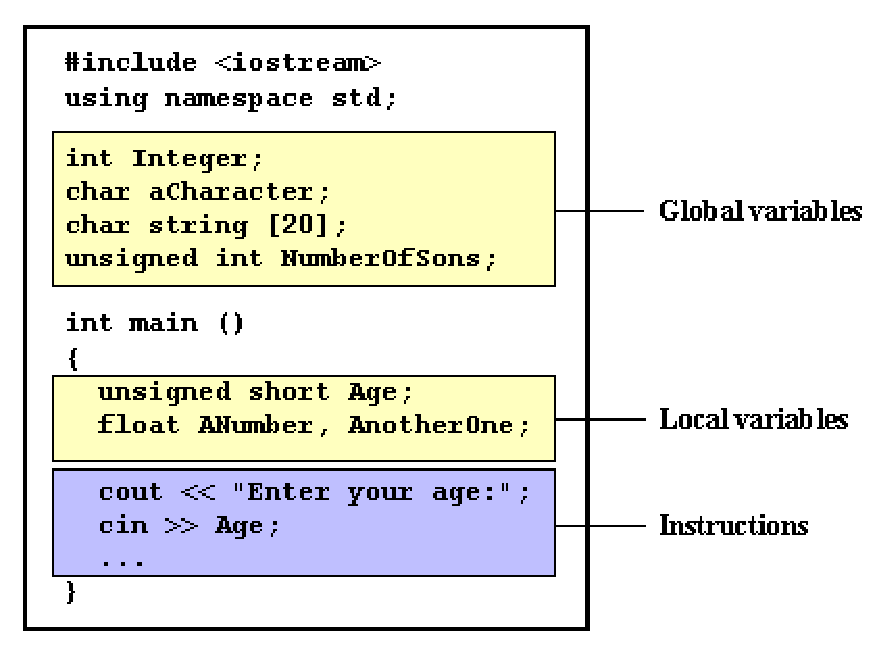
\includegraphics[height=40mm]{./figs/variable_scope.eps}
				\caption{Variable scope\footnotemark.}
			\end{figure}
	  \end{column}
	\end{columns}
	\footnotetext{Source: \url{http://www.cplusplus.com/doc/tutorial/variables/}.}
	\pause
  \dontblock{Declare variables in global scope.  Limit the scope as much as possible to reduce chance of side-effects.  Global constants, however, are fine.}
	

\end{frame}

\section{Operators}

\begin{frame}[fragile]
 \frametitle{Simple operators}
 \begin{block}{Assignment: \texttt{=}}
    \begin{lstlisting}
  a = 5; a = b;
   \end{lstlisting}
  \end{block}
  \pause
  \begin{block}{Arithmetic operators: \texttt{+, -, *, /, \%}}
   All obvious with the exception of the \textit{modulo} operator (\texttt{\%}).  This gives the remainder after division e.g.
  \begin{lstlisting}
  a = 22 % 7;
  \end{lstlisting}
  will set \texttt{a} to \text{1} as $\frac{22}{7} = 3 \times 7 \text{ remainder } 1$.
 \end{block}
 \pause
 \begin{block}{Compound assignment: \texttt{+=, -=, *=, /=, \%=}}
  Perform the operation on the current value of the variable and then set it to the new value, e.g.:
  \begin{lstlisting}
  a += 5; a *= b;
  \end{lstlisting}
 \end{block} %end item
\end{frame}


\begin{frame}[fragile]
  \frametitle{Integer arithmetic}
  
  \begin{warnblocke}
  	In C++ \emph{integer} arithmetic truncates (effectively rounds down):
  	\begin{lstlisting}
  int a = 20;
  int b = 7;
  int someInteger = a / b; // = 2
  	\end{lstlisting}
  	Storing the result in a double doesn't help as the arithmetic has already been done:
  	\begin{lstlisting}
  double someDouble = a / b; // = 2
  double anotherDouble = 20/7; // = 2
  	\end{lstlisting}
  \end{warnblocke}
  	What gives?\\
  	\pause{}  To get around we can ``cast'' the variable to another type:
  	\begin{enumerate}
  	  \item{
  	  	\begin{lstlisting}
someDouble = static_cast<double>(dividend) /
  static_cast<double>(divisor); // = 2.85714
  	  	\end{lstlisting}}
  	  \item{
  	  	\begin{lstlisting}
anotherDouble = 20./7.; // = 2.85714
  	  	\end{lstlisting}}
  	  
  	\end{enumerate}

\end{frame}

\begin{frame}[fragile]
  \begin{block}{Unary operators: \texttt{++, --}}
    \begin{lstlisting}
  a++;
   \end{lstlisting}
   This is equivalent to:
   \begin{lstlisting}
  a += 1;
   \end{lstlisting}
  \end{block}
  \pause
  \begin{block}{Relational and equality operators: \texttt{==, !=, >, <, >=, <=}}
  Evaluates to a boolean (true or false) value e.g.:
    \begin{lstlisting}
  bool areNotEqual = (a != b);
   \end{lstlisting}
 \end{block}
 \pause
 \begin{dontblocke}%
 Mix up \texttt{=} and \texttt{==} this will cause endless headaches!  Consider:
 \begin{lstlisting}
  a = 5; b = 6; areEqual = (a = b);
 \end{lstlisting}
 This is a problem because C++ considers any number other than 0 be true!
 \end{dontblocke}
\end{frame}

\begin{frame}[fragile]
  \begin{block}{Logical operators: \texttt{!, \&\&, ||}}
    These act on boolean values in the following ways:
    \begin{columns}[t]
      \begin{column}[T]{0.2\linewidth}
        NOT
        \begin{tabular}{c|c}
          a & !a \\
          \hline
          \kw{true} & \kw{false} \\
          \kw{false} & \kw{true}
        \end{tabular}
		  \end{column}
		  \begin{column}[T]{0.3\linewidth}
		    AND
		    \begin{tabular}{c|c|c}
		    a & b & a \texttt{\&\&} b \\
		    \hline
		    \kw{true} & \kw{true} & \kw{true} \\
		    \kw{true} & \kw{false} & \kw{false} \\
		    \kw{false} & \kw{true} & \kw{false} \\
		    \kw{false} & \kw{false} & \kw{false}
		    \end{tabular}
      \end{column}
		  \begin{column}[T]{0.3\linewidth}
		    OR
		    \begin{tabular}{c|c|c}		
		    a & b & a \texttt{||} b \\
		    \hline
		    \kw{true} & \kw{true} & \kw{true} \\
		    \kw{true} & \kw{false} & \kw{true} \\
		    \kw{false} & \kw{true} & \kw{true} \\
		    \kw{false} & \kw{false} & \kw{false}
		    \end{tabular}
      \end{column}
    \end{columns}
  \end{block}
  \pause
  \begin{doblocke}
  Keep it simple: don't try and do too much in a single line.  While this:
  \begin{lstlisting}
    result = (i < 10) && (++i < n);
  \end{lstlisting}
  is a valid expression, deciphering what it does is a lot of work.  Instead use:%
  \begin{lstlisting}
    result = i < 10;
    ++i;
    result = result && i < n;
  \end{lstlisting}
%TODO: Check above is true
  \end{doblocke}
\end{frame}

\begin{frame}[fragile]
  \frametitle{Operator precedence}
  \framesubtitle{No, you got first...}
  \begin{columns}[t]
	  \begin{column}[T]{0.44\textwidth}
		  \begin{tabular}{c|l|m{2.1cm}}
			  Precedence & Op. & Associativity \\
			  \hline
			  \multirow{2}{*}{1} & \texttt{++ --} & \multirow{2}{*}{Left to Right}\\
			    & \texttt{!} \\
			  \hline
			  2 & \texttt{* / \%} & \multirow{6}{*}{Left to Right} \\
			  \cline{1-2}
			  3 & \texttt{+ -} & \\
			  \cline{1-2}
			  \multirow{2}{*}{4} & \texttt{< <=} \\
			    & \texttt{> >=} \\
			  \cline{1-2}
			  5 & \texttt{== !=} \\
			  \cline{1-2}
			  6 & \texttt{\&\&} \\
			  \cline{1-2}
			  7 & \texttt{||} \\
			  \hline
			  8 & \texttt{=} & Right to Left
		  \end{tabular}
	 	\end{column}
  	\begin{column}[T]{0.38\textwidth}
	  Operator precedence tells you the order that an expression will be evaluated in.  Some are obvious but consider:
	  \begin{lstlisting}
  a = 21 + 7 % 2;
	  \end{lstlisting}
    which could be interpreted as
	  \begin{lstlisting}
  a = 21 + (7 % 2); // this
  a = (21 + 7) % 2; // or this.
	  \end{lstlisting}
	  In fact the first version is correct.
	  
  	\end{column}
 	\end{columns}
\end{frame}
\begin{frame}
	\doblock{Use parentheses to make an expressions more clear even if they are not necessary.}
\end{frame}

\begin{frame}[fragile]
  \frametitle{Operator precedence}
  \framesubtitle{No, you got first...}
  \begin{columns}[t]
	  \begin{column}[T]{0.44\textwidth}
		  \begin{tabular}{c|l|m{2.1cm}}
			  Precedence & Op. & Associativity \\
			  \hline
			  \multirow{2}{*}{1} & \texttt{++ --} & \multirow{2}{*}{Left to Right}\\
			    & \texttt{!} \\
			  \hline
			  2 & \texttt{* / \%} & \multirow{6}{*}{Left to Right} \\
			  \cline{1-2}
			  3 & \texttt{+ -} & \\
			  \cline{1-2}
			  \multirow{2}{*}{4} & \texttt{< <=} \\
			    & \texttt{> >=} \\
			  \cline{1-2}
			  5 & \texttt{== !=} \\
			  \cline{1-2}
			  6 & \texttt{\&\&} \\
			  \cline{1-2}
			  7 & \texttt{||} \\
			  \hline
			  8 & \texttt{=} & Right to Left
		  \end{tabular}
	 	\end{column}
	  \begin{column}[T]{0.38\textwidth}
	     Operators that have the same precedence are evaluated according to their \textit{associativity} e.g.:
	    \begin{lstlisting}
	a = b = c;   // evaluates as
	a = (b = c);
	    \end{lstlisting}
			because \texttt{=} is right to left associative. 
			\pause  While:
	    \begin{lstlisting}
	a * b % c;
	//evaluates as
	(a * b) % c;
	    \end{lstlisting}
	 are left to right associative. 
	    
	  \end{column}
	\end{columns}
\end{frame}


\section{Basic input and output}

\begin{frame}[fragile]
  \frametitle{Standard output (\texttt{cout})}
  
  You've already met \texttt{cout}, it uses the \textit{indirection operator} (\texttt{<<}) to print to the screen e.g.:
  \begin{lstlisting}
std::cout << "Have some pi: ";
std::cout << 3.1415926;
std::cout << a;
  \end{lstlisting}
  \pause
  We can use \texttt{<<} more than once in the same statement:
  \begin{lstlisting}
double t0 = 1.5, t1 = 2.5;
cout << "t0: " << t0 << ", t1: " << t1
     << ", delta: " << t1 - t0;
  \end{lstlisting}
	\cout{t0: 1.5, t1: 2.5, delta: 1}
	\newline\pause
  If you want a new line you have to use \texttt{\char`\\ n}:
  \begin{lstlisting}
double t0 = 1.5, t1 = 2.5;
cout << "t0: " << t0 << "\nt1: " << t1 << "\n";
  \end{lstlisting}
  \cout{t0: 1.5 \newline t1: 2.5}
% TODO: Change output so it looks alright!
\end{frame}

\begin{frame}[fragile]
  \frametitle{Standard input (\texttt{cin})}
  \framesubtitle{Extracting information out of the user}
  To get input from the user, use the extraction operator (\texttt{>>}) of the \texttt{cin} object (pronounced \textit{see-in}) e.g.:
  \begin{lstlisting}
  double radius;
  std::cin >> radius;
  \end{lstlisting}
  at this point the program will stop and wait for the user to enter a number and push RETURN.
  \pause
  As with output we can use \texttt{>>} more than once in a statement e.g.:
  \begin{lstlisting}
  std::cin >> width >> height;
  \end{lstlisting}
  in this case the program will wait for two sets of numbers to be entered.  They can be separated by a space, tab or a newline.
\end{frame}

\begin{frame}[fragile]
  \frametitle{Complete example}
  \framesubtitle{Putting it all together}
  \lstinputlisting[language=C++,title=\lstsrctitle]{../code/0_basics/lectures/rect_info.cpp}
\end{frame}


\end{document}
\documentclass{beamer}
%\documentclass[handout]{beamer}

% Input all common stuff


% THEME SETTINGS %%%%%%%%%%%%
\usetheme[secheader]{Boadilla}
\usecolortheme{default}
\useinnertheme{circles}
\setbeamertemplate{blocks}[default]

% Get rid of bottom navigation bars
\setbeamertemplate{footline}[page number]{}

% Gets rid of navigation symbols
\setbeamertemplate{navigation symbols}{}

% PACKAGES %%%%%%%%%%%%%%%%%%%
\usepackage{listings}
\usepackage{xcolor}
\usepackage{multirow}
\usepackage{array}
\usepackage{verbatim}
\usepackage{pbox}
\usepackage{tabularx}

% LISTINGS STYLE %%%%%%%%%%%%%
\definecolor{bluekeywords}{rgb}{0.13,0.13,1}
\definecolor{greencomments}{rgb}{0,0.5,0}
\definecolor{redstrings}{rgb}{0.9,0,0}
\definecolor{listingsbg}{HTML}{EFEFFF}

\lstset{language=C++,
  showspaces=false,            % show spaces adding particular underscores
  showtabs=false,              % show tabs within strings adding particular underscores
  breaklines=true,             % sets automatic line breaking
  showstringspaces=false,      % underline spaces within strings
  breakatwhitespace=true,      % sets if automatic breaks should only happen at whitespace
  captionpos=b,                % sets the caption-position to bottom
  escapeinside={(*@}{@*)},
  commentstyle=\color{greencomments},
  keywordstyle=\color{bluekeywords}\bfseries,
  stringstyle=\color{redstrings},
  basicstyle=\ttfamily\fontsize{9}{10}\selectfont,
  backgroundcolor=\color{listingsbg}
}

% MACROS %%%%%%%%%%%%%%%%%%%%%
\newcommand{\lstsrctitle}[0]{%
 {\scriptsize\lstname}
}

\newcommand{\kw}[1]{\texttt{\textcolor{bluekeywords}{\ttfamily\fontsize{9}{10}\selectfont #1}}}

\newenvironment{varblock}[3]{%
  \setbeamercolor{block body}{#2}
  \setbeamercolor{block title}{#3}
  \begin{block}{#1}}{\end{block}}

% Colours taken from http://twitter.github.com/bootstrap/components.html#alerts
% Do block %%%%%%%%%%%%%%%%%%%%%%
\definecolor{doblocktext}{HTML}{468847}
\definecolor{doblockbg}{HTML}{DFF0D8}
\newenvironment{doblocke}[0]{% begin
  \begin{varblock}{\textbf{Do}}%
  {bg=doblockbg,fg=doblocktext}{bg=doblocktext,fg=white}%
  \setbeamercolor{itemize item}{fg=doblocktext}
  \lstset{backgroundcolor=}% The background should be the same as that of the block
  } % begin
  {\end{varblock}} %end
  
\newcommand{\doblock}[1]{%
 \begin{doblocke}#1\end{doblocke} 
}

% Don't block %%%%%%%%%%%%%%%%%%%
\definecolor{dontblocktext}{HTML}{B94A48}
\definecolor{dontblockbg}{HTML}{F2DEDE}  
\newenvironment{dontblocke}[0]{% begin
  \begin{varblock}{\textbf{Don't}}%
  {bg=dontblockbg,fg=dontblocktext}{bg=dontblocktext,fg=white}
  \setbeamercolor{itemize item}{fg=dontblocktext}
  \lstset{backgroundcolor=}% The background should be the same as that of the block
  }%
  {\end{varblock}} %end

\newcommand{\dontblock}[1]{%
 \begin{dontblocke}#1\end{dontblocke} 
}

% Defi block %%%%%%%%%%%%%%%%%%%%
\definecolor{defiblocktext}{HTML}{3A87AD}
\definecolor{defiblockbg}{HTML}{D9EDF7}
\newenvironment{defiblocke}[1]{% begin
  \begin{varblock}{\textbf{Definition}}%
  {bg=defiblockbg,fg=defiblocktext}{bg=defiblocktext,fg=white}
  \lstset{backgroundcolor=}% The background should be the same as that of the block
  \textit{#1} }
  {\end{varblock}} %end

\newcommand{\defiblock}[2]{%
 \begin{varblock}{\textbf{Definition}}%
 {bg=defiblockbg,fg=defiblocktext}{bg=defiblocktext,fg=white}%
  \begin{tabularx}{\linewidth}{lX}\textit{#1} & #2\end{tabularx}
 \end{varblock} 
}

\newenvironment{defiblockbaree}[1]{ %begin
  \begin{varblock}{\textbf{#1}}%
  {bg=defiblockbg,fg=defiblocktext}{bg=defiblocktext,fg=white}
  \lstset{backgroundcolor=}} %begin
  {\end{varblock}} %end

\definecolor{warnblocktext}{HTML}{C09853}
\definecolor{warnblockbg}{HTML}{FCF8E3}
\newenvironment{warnblocke}[0]{% begin
  \begin{varblock}{\textbf{Warning!}}%
  {bg=warnblockbg,fg=warnblocktext}{bg=warnblocktext,fg=white}
  \lstset{backgroundcolor=}% The background should be the same as that of the block
  \setbeamercolor{itemize item}{fg=warnblocktext}
  \setbeamercolor{item projected}{fg=white,bg=warnblocktext}
  } % begin
  {\end{varblock}} % end

\newcommand{\warnblock}[1]{%
  \begin{warnblocke}#1\end{warnblocke}
} % newcommand

\newcommand{\cout}[1]{%
 Output: \pbox[t]{\textwidth}{\ttfamily\fontsize{9}{10}\selectfont{}#1}
}

\newenvironment{doitemize}[0]{%
  \begin{itemize}}%
  {\end{itemize}} %end


% CONSTANTS %%%%%%%%%%%%%%%%%%%%%%%%%%%

%Symbol for backslash in texttt \char`\\

% Common title slide stuff
\title{Introduction to Scientific Programming with C++}
\author{Martin Uhrin}
\institute{UCL}
\date{February 11-13th 2013}

\subtitle{Session 1: Control structure}

\begin{document}

\frame{\titlepage}

\begin{frame}
\frametitle{Table of Contents}
\tableofcontents
\end{frame}

\section{Conditionals}

\begin{frame}[fragile]
	\frametitle{if, else}
	So far our programs have been linear: one start, one end, one path in between.  Let's branch out:
	\pause
	\begin{lstlisting}
if(speed == 88){std::cout << "Great Scott!";}
	\end{lstlisting}
	the statement after the \texttt{if} condition will only be executed if the condition is true.\pause  You can execute more than one statment within a \texttt{\{ \}} block:
	\begin{lstlisting}
if(power >= 1.21)
{
  std::cout << "1.21 gigawatts!";
  std::cout << "1.21 gigawatts. Great Scott!\n";
}
	\end{lstlisting} 
	\pause
	We can also specify what to do if the condition is not fulfilled:
	\begin{lstlisting}
bool haveEnoughPower;
if(power >= 1.21){
  haveEnoughPower = true;
}else{
  haveEnoughPower = false;
}
	\end{lstlisting}
\end{frame}



\begin{frame}[fragile]
  \frametitle{if, else}
  Lastly we can string together a series of conditionals, like so:
	\begin{lstlisting}
int width, height;
std::cin >> width >> height;
	
if(width > height){
  std::cout << "Fat rectangle\n";
}else if(height > width){
  std::cout << "Tall rectangle\n";
}else if(width == height){
  std::cout << "Square\n";
}else{
  std::cout << "IMPOSSIBLE!!";
}
	\end{lstlisting}
	These are evaluated one after another until one is found to be true, otherwise the final \kw{else} statement is executed.
	\pause
	\doblock{Keep conditionals simple, break them up if you have to.  A huge proportion of programming errors come from conditional statements.}
\end{frame}

\section{Loops}

\subsection{while loops}

\begin{frame}[fragile]
  \frametitle{Loops}
  The purpose of a loop is to execute a set of statements until a condition is fulfilled.
  \pause
  \begin{block}{while loop}
    \begin{lstlisting}
while(expression) statement
    \end{lstlisting}
    Example:
  \begin{lstlisting}
  int t = 10;
  while(t != 0)
  {
    std::cout << t << ", ";
    --t;  
  }
  std::cout << "Blastoff!";
  \end{lstlisting}
  \end{block}
\end{frame}

\subsection{do-while loops}

\begin{frame}[fragile]
  \frametitle{Loops}
  \framesubtitle{Go on, go on, go on, go on, go on...}
  
  \begin{block}{do-while loop}
    \begin{lstlisting}
do statement while(expression);
    \end{lstlisting}
    \lstinputlisting[language=C++,title=\lstsrctitle,belowskip=0pt]%
    {../code/1_control_structure/lectures/tea_father.cpp}
  \end{block}
\end{frame}

\subsection{for loops}

\begin{frame}[fragile]
  \frametitle{Loops}
  
  \begin{block}{for loop}
    \begin{lstlisting}
  for(initialisation; condition; increment) statement;
    \end{lstlisting}
    This works as follows:
    \begin{enumerate}
      \item<2->{\texttt{initialisation} is executed.  Usually used to initialise a counter.  This happens once.}
      \item<3->{\texttt{condition} is checked, if true the loop continues, otherwise the loop ends and is skipped.}
      \item<4->{\texttt{statement} is executed.}
      \item<5->{\texttt{increment} is executed and we go back to step 2.}
    \end{enumerate}
\end{block}
    \pause[6]
    Here's our blastoff example with a for loop:
    \begin{lstlisting}[belowskip=0pt]
  for(int t = 10; t <= 0; --t)
  {
    std::cout << t << ", ";
  }
  std::cout << "Blastoff!";
    \end{lstlisting}
    
  
\end{frame}

\section{Functions}

\begin{frame}[fragile]
  \frametitle{Functions}
  \framesubtitle{How would we function without them?}
  Functions provide a way of structuring a program in a more modular way, by grouping sets of statement so they can be easily reused.\newline
  \pause
  Consider: what if we want to calculate gravitational force between multiple bodies?
  \begin{lstlisting}
forceEarthSun = G * massEarth * massSun /
  (rEarthSun * rEarthSun);
forceEarthMoon = G * massEarth * massMoon /
  (rEarthMoon * rEarthMoon);
forceEarthMars = G * massEarth * massMars /
  (rEarthMars * rEarthMars);
  \end{lstlisting}
  \pause
  wouldn't it be better to be able to write:
  \begin{lstlisting}
forceEarthSun = force(massEarth,  massSun, rEarthSun);
forceEarthMoon = force(massEarth, massMoon, rEarthMoon);
forceEarthMars = force(massEarth, massMars, rEarthMars);
  \end{lstlisting}
  Through the magic of functions, we can!
\end{frame}


\begin{frame}[fragile]
  \frametitle{Functions}

  Format of a function:
  \begin{lstlisting}
type name(parameter1, parameter2, ...) { statements }  
  \end{lstlisting}
  where:
  \begin{itemize}
    \item<2->{\texttt{type} is the data type that is returned to you by the function.}
    \item<3->{\texttt{name} is the unique identifier (name) of the function.}
    \item<4->{\texttt{parameter}, each of these is just like a variable definition (e.g. \texttt{\kw{double} mass}).}
    \item<5->{\texttt{statements} are the function's \textit{body}.  These statements will execute when the function is called.}
  \end{itemize}
  \pause[6]
  Let's try:
  \begin{lstlisting}
double force(const double mass1, const double mass2,
  const double r)
{
  return G * mass1 * mass2 / (r * r);
}
  \end{lstlisting}
\end{frame}


\begin{frame}[fragile]
  \frametitle{Functions}

  Let's try a full example:
  \lstinputlisting[language=C++,basicstyle=\ttfamily\fontsize{7}{8}\selectfont,title=\lstsrctitle]{../code/1_control_structure/lectures/grav_force.cpp}
\end{frame}

\begin{frame}
  \frametitle{Function nomenclature}
  
  \defiblock{caller}{A point in code that \textit{calls} a function.  A value is said to be \text{returned} to the caller when the function finishes.}
  
\end{frame}

\begin{frame}[fragile]
  \frametitle{Functions with no type}
  
  What if we want to have a function that doesn't return anything?\newline
  \pause
  Use \kw{void}:
  \begin{lstlisting}
void printForce(const std::string object1,
  const std::string object2,
  const double force)
{
  std::cout << object1 << " " << object2 << ":" << force << "\n";
}
  \end{lstlisting}
  In C++ \kw{void} denotes the absence of a type.
\end{frame}

\subsection{Declaring functions}

\begin{frame}[fragile]
  \frametitle{Declaring functions}
  \framesubtitle{I do declare}
  
  All identifiers have to be declared before they are used.  So how are we to code something like:
  \begin{lstlisting}
const bool ON = true, OFF = false
const bool OPEN = true, CLOSED = false;

void setMicrowaveState(const bool newState) {
  if(newState == ON)
  {
    setMicrowaveDoor(CLOSED); // <- ERROR: Don't know about 
    state = ON;               // setMicrowaveDoor 
  }
  else
  	state = OFF;
}
void setMicrowaveDoor(const bool newState) {
  if(newState == OPEN)
    setMicrowaveState(OFF);

  doorState = newState;
}
  \end{lstlisting}
\end{frame}


\begin{frame}[fragile]
  \frametitle{Declaring functions}
  \framesubtitle{I do declare}
  
  To get around this declare the \texttt{setMicrowaveDoor} function before \texttt{setMicrowaveState} like this:
  \begin{lstlisting}
void setMicrowaveDoor(const bool newState);

void setMicrowaveState(const bool newState) {
  if(newState == ON)
  {
    setMicrowaveDoor(CLOSED); // Happy: you've told me about
    state = ON;               // setMicrowaveDoor
  }
  ...
}
void setMicrowaveDoor(const bool newState) { /*as before*/ }
  \end{lstlisting}
  The first line tells the compiler: expect to see a \texttt{setMicrowaveDoor} function somewhere further down, and this is what it will look like.
\end{frame}

\begin{frame}[fragile]
  \frametitle{Declaring functions}
  \begin{defiblocke}{function prototype}%
The header of a function without any of the body. Used in function declarations, e.g.:
    \begin{lstlisting}
void setMicrowaveDoor(const bool newState);
    \end{lstlisting}
  \end{defiblocke}
\end{frame}

\subsection{Default values}

\begin{frame}[fragile]
  \frametitle{Default values}
  \defiblock{default value}{A value that is used as a function parameter if the caller doesn't supply one.}
	An example:
	
  \begin{columns}[t]
    \begin{column}[T]{0.48\textwidth}
    \lstinputlisting[language=C++,title=\lstsrctitle,linerange={3-13},basicstyle=\ttfamily\fontsize{8}{9}\selectfont]{../code/1_control_structure/lectures/dispense_drink.cpp}  
    \end{column}
    \begin{column}[T]{0.48\textwidth}
\lstinputlisting[language=C++,firstline=15,basicstyle=\ttfamily\fontsize{8}{9}\selectfont]{../code/1_control_structure/lectures/dispense_drink.cpp}  
	  \end{column}
	\end{columns}
\end{frame}

\begin{frame}[fragile]
  \frametitle{Default values}
  
  Default values have to be at the end of the parameter list, e.g.:
  \begin{lstlisting}
void dispenseDrink(int size,
  int drinkType = COFFEE,
  bool withMilk = false) { ... } // Good, can call:
  
dispenseDrink(1);      // or ...
dispenseDrink(3, TEA); // or ...
dispenseDrink(2, COFFEE, true)
  \end{lstlisting}
  \pause
  Bad:
  \begin{lstlisting}
void dispenseDrink(int drinkType = COFFEE,
  int size,
  bool withMilk = false) { ... }
  
dispenseDrink(/*what goes here?*/, 2); // Error!
  \end{lstlisting}
\end{frame}

\begin{frame}[fragile]
  \frametitle{Default values}
  
  \begin{doblocke}
    \begin{doitemize}
      \item{Use default values to automate commonly used parameter values or provide the user with optional parameters.}
      \pause
      \item{To give an indication of what a reasonable parameter value might be.}
    \end{doitemize}
  \end{doblocke}
\end{frame}

\subsection{Overloading functions}

\begin{frame}[fragile]
  \frametitle{Overloading functions}
  
  What if you want to create a dot product function that works for both integers and doubles?  Could write:
  \begin{lstlisting}
int dotInt(int x0, int y0, int x1, int y1)
{ return x0 * x1 + y0 * y1; }
double dotDouble(double x0, double y0, double x1, double y1)
{ return x0 * x1 + y0 * y1; }

dotInt(fromX, fromY, toX, toY);
  \end{lstlisting}
  Have to look up which dot function to call based on my number type. Ideally I'd like to call \texttt{dot} and let the compiler choose the right one.
  \newline\pause
  No problem, use:
  \begin{lstlisting}[belowskip=0pt]
int dot(int x0, int y0, int x1, int y1)
{ return x0 * x1 + y0 * y1; }
double dot(double x0, double y0, double x1, double y1)
{ return x0 * x1 + y0 * y1; }

dot(fromX, fromY, toX, toY); // Compiler will choose
                             // correct version based on
                             // from/to number types
  \end{lstlisting}
\end{frame}

\begin{frame}[fragile]
  \frametitle{Overloading functions}
  
  \defiblock{overloaded functions}{two or more functions with the same name but different parameter types and/or numbers of parameters.}
  \pause
  Examples:
  \begin{lstlisting}
// Sum two or three integers
int sum(int n1, int n2);
int sum(int n1, int n2, int n3);

// Add together any integer/double
int add(int n1, int n2);
double add(int n1, double n2);
double add(double n1, int n2);
double add(double n1, double n2);
  \end{lstlisting}  

\end{frame}

\subtitle{Inbuilt math functions}

\begin{frame}[fragile]
  \frametitle{Math functions}
  \framesubtitle{C numerics library}
  
  As scientists we're going to want to manipulate numbers.  Here are some commonly used functions that are available as part of the \texttt{cmath} header:
  
	  \begin{tabularx}{\linewidth}{XX}
		  \texttt{abs} & absolute value \\
		  \texttt{sin, cos, tan} & Warning: take angle in radians! \\
		  \texttt{exp, log, log10} & raise $e$ to power, natural log and base 10 log \\
		  \texttt{sqrt} & \\
		  \texttt{pow(\kw{double} base, \kw{double} exp)} & raise \texttt{based} to power \texttt{exp} 
	  \end{tabularx}
  \newline
  See \footnote{\url{http://www.cplusplus.com/reference/clibrary/cmath/}} for a full list.
  \newline
	\pause
  To use the math functions include the cmath header by writing:
  \begin{lstlisting}
#include <cmath>
  \end{lstlisting}
  at the start of you program.
\end{frame}

\subsection{Recursive functions}

\begin{frame}[fragile]
  \frametitle{Recursivity}
  \defiblock{recursive function}{a function that calls itself.}
  This is similar to a recurrence relation in mathematics e.g.:
  \begin{equation*}
  b_n = n b_{(n - 1)}, b_0 = 1
  \end{equation*}
  which gives the factorial of a number ($n!$).\pause{}  And in C++:
  \lstinputlisting[language=C++,title=\lstsrctitle,firstline=3,lastline=9]{../code/1_control_structure/lectures/factorial.cpp}  
  
\end{frame}

\end{document}

\documentclass{beamer}
%\documentclass[handout]{beamer}

% Input all common stuff


% THEME SETTINGS %%%%%%%%%%%%
\usetheme[secheader]{Boadilla}
\usecolortheme{default}
\useinnertheme{circles}
\setbeamertemplate{blocks}[default]

% Get rid of bottom navigation bars
\setbeamertemplate{footline}[page number]{}

% Gets rid of navigation symbols
\setbeamertemplate{navigation symbols}{}

% PACKAGES %%%%%%%%%%%%%%%%%%%
\usepackage{listings}
\usepackage{xcolor}
\usepackage{multirow}
\usepackage{array}
\usepackage{verbatim}
\usepackage{pbox}
\usepackage{tabularx}

% LISTINGS STYLE %%%%%%%%%%%%%
\definecolor{bluekeywords}{rgb}{0.13,0.13,1}
\definecolor{greencomments}{rgb}{0,0.5,0}
\definecolor{redstrings}{rgb}{0.9,0,0}
\definecolor{listingsbg}{HTML}{EFEFFF}

\lstset{language=C++,
  showspaces=false,            % show spaces adding particular underscores
  showtabs=false,              % show tabs within strings adding particular underscores
  breaklines=true,             % sets automatic line breaking
  showstringspaces=false,      % underline spaces within strings
  breakatwhitespace=true,      % sets if automatic breaks should only happen at whitespace
  captionpos=b,                % sets the caption-position to bottom
  escapeinside={(*@}{@*)},
  commentstyle=\color{greencomments},
  keywordstyle=\color{bluekeywords}\bfseries,
  stringstyle=\color{redstrings},
  basicstyle=\ttfamily\fontsize{9}{10}\selectfont,
  backgroundcolor=\color{listingsbg}
}

% MACROS %%%%%%%%%%%%%%%%%%%%%
\newcommand{\lstsrctitle}[0]{%
 {\scriptsize\lstname}
}

\newcommand{\kw}[1]{\texttt{\textcolor{bluekeywords}{\ttfamily\fontsize{9}{10}\selectfont #1}}}

\newenvironment{varblock}[3]{%
  \setbeamercolor{block body}{#2}
  \setbeamercolor{block title}{#3}
  \begin{block}{#1}}{\end{block}}

% Colours taken from http://twitter.github.com/bootstrap/components.html#alerts
% Do block %%%%%%%%%%%%%%%%%%%%%%
\definecolor{doblocktext}{HTML}{468847}
\definecolor{doblockbg}{HTML}{DFF0D8}
\newenvironment{doblocke}[0]{% begin
  \begin{varblock}{\textbf{Do}}%
  {bg=doblockbg,fg=doblocktext}{bg=doblocktext,fg=white}%
  \setbeamercolor{itemize item}{fg=doblocktext}
  \lstset{backgroundcolor=}% The background should be the same as that of the block
  } % begin
  {\end{varblock}} %end
  
\newcommand{\doblock}[1]{%
 \begin{doblocke}#1\end{doblocke} 
}

% Don't block %%%%%%%%%%%%%%%%%%%
\definecolor{dontblocktext}{HTML}{B94A48}
\definecolor{dontblockbg}{HTML}{F2DEDE}  
\newenvironment{dontblocke}[0]{% begin
  \begin{varblock}{\textbf{Don't}}%
  {bg=dontblockbg,fg=dontblocktext}{bg=dontblocktext,fg=white}
  \setbeamercolor{itemize item}{fg=dontblocktext}
  \lstset{backgroundcolor=}% The background should be the same as that of the block
  }%
  {\end{varblock}} %end

\newcommand{\dontblock}[1]{%
 \begin{dontblocke}#1\end{dontblocke} 
}

% Defi block %%%%%%%%%%%%%%%%%%%%
\definecolor{defiblocktext}{HTML}{3A87AD}
\definecolor{defiblockbg}{HTML}{D9EDF7}
\newenvironment{defiblocke}[1]{% begin
  \begin{varblock}{\textbf{Definition}}%
  {bg=defiblockbg,fg=defiblocktext}{bg=defiblocktext,fg=white}
  \lstset{backgroundcolor=}% The background should be the same as that of the block
  \textit{#1} }
  {\end{varblock}} %end

\newcommand{\defiblock}[2]{%
 \begin{varblock}{\textbf{Definition}}%
 {bg=defiblockbg,fg=defiblocktext}{bg=defiblocktext,fg=white}%
  \begin{tabularx}{\linewidth}{lX}\textit{#1} & #2\end{tabularx}
 \end{varblock} 
}

\newenvironment{defiblockbaree}[1]{ %begin
  \begin{varblock}{\textbf{#1}}%
  {bg=defiblockbg,fg=defiblocktext}{bg=defiblocktext,fg=white}
  \lstset{backgroundcolor=}} %begin
  {\end{varblock}} %end

\definecolor{warnblocktext}{HTML}{C09853}
\definecolor{warnblockbg}{HTML}{FCF8E3}
\newenvironment{warnblocke}[0]{% begin
  \begin{varblock}{\textbf{Warning!}}%
  {bg=warnblockbg,fg=warnblocktext}{bg=warnblocktext,fg=white}
  \lstset{backgroundcolor=}% The background should be the same as that of the block
  \setbeamercolor{itemize item}{fg=warnblocktext}
  \setbeamercolor{item projected}{fg=white,bg=warnblocktext}
  } % begin
  {\end{varblock}} % end

\newcommand{\warnblock}[1]{%
  \begin{warnblocke}#1\end{warnblocke}
} % newcommand

\newcommand{\cout}[1]{%
 Output: \pbox[t]{\textwidth}{\ttfamily\fontsize{9}{10}\selectfont{}#1}
}

\newenvironment{doitemize}[0]{%
  \begin{itemize}}%
  {\end{itemize}} %end


% CONSTANTS %%%%%%%%%%%%%%%%%%%%%%%%%%%

%Symbol for backslash in texttt \char`\\

% Common title slide stuff
\title{Introduction to Scientific Programming with C++}
\author{Martin Uhrin}
\institute{UCL}
\date{February 11-13th 2013}

\subtitle{Session 2: More data types}

\begin{document}

\frame{\titlepage}

\begin{frame}
\frametitle{Table of Contents}
\tableofcontents
\end{frame}


\section{Arrays}

\subsection{Declaring arrays}

\begin{frame}[fragile]
	\frametitle{Arrays}
	
	\defiblock{array}{a series of elements of the same type occupying a contiguous block of memory.}
	
	Format for declaring an array is:
	\begin{lstlisting}
	type name[num_elements];
	\end{lstlisting}
	Where \texttt{type} is any valid data type and \texttt{num\_elements} is a constant positive integer.
	\pause
	Some examples:
	\begin{lstlisting}
	unsigned int lotteryNumbers[7];
	
	double planetMasses[8];
	
	const unsigned int numParticles = 128;
	double xPositions[numParticles];
	double yPositions[numParticles];
	\end{lstlisting}
	Last example shows how we can use constant variable as array size.
	
\end{frame}

\subsection{Using arrays}

\begin{frame}[fragile]
  \frametitle{Initialising arrays}
  When declaring an array it can be initialised as follows:
  \begin{lstlisting}
unsigned int lotteryNumbers[7] = {16, 3, 28, 9, 24, 10, 8}
  \end{lstlisting}
  the size can be left out, in which case the number of values given is used:
  \begin{lstlisting}
unsigned int lotteryNumbers[] = {16, 3, 28, 9, 24, 10, 8}
  \end{lstlisting}  
\end{frame}

\begin{frame}[fragile]
  \frametitle{Accessing elements}
  
  To access an element of an array the format is:
  \begin{lstlisting}
  name[index]
  \end{lstlisting}
  \warnblock{In C++ array numbering starts at 0!  This is a huge source of confusion especially if you're used to a programming language like Fortran where arrays start at 1.}
  \pause
  For example, to read the 3$^{rd}$ lottery number use:
  \begin{lstlisting}
  unsigned int third = lotteryNumbers[2];
  \end{lstlisting}
  \pause
  To write the 3$^{rd}$ lottery number use:
  \begin{lstlisting}
  lotteryNumber[2] = 23;
  \end{lstlisting}
  \pause
  You can also access the elements using a variable:
  \begin{lstlisting}
  for(int i = 0; i < 7; ++i)
     std::cout << lotteryNumbers[i] << " ";
  \end{lstlisting}
\end{frame}

\begin{frame}[fragile]
  \frametitle{Accessing elements}
  \framesubtitle{Array index out of bounds}
    \begin{warnblocke}Be careful not to access elements past the end of an array.  Consider:
    \begin{lstlisting}
  const unsigned int numPlanets = 8;
  double masses[numPlanets];
  for(int i = 0; i <= numPlanets; ++i)
    masses[i] = random();
    \end{lstlisting}
	Seems ok, but wait.  The last iteration will try to set \texttt{masses[8]} which is past the end of the array!
    \end{warnblocke}

\end{frame}

\subsection{Multidimensional arrays}

\begin{frame}[fragile]
  \frametitle{Multidimensional arrays}
  \framesubtitle{Because with only two friends 1D is sooo boring}
  Think of multidimensional arrays as being "arrays of arrays".  An example:
  \lstinputlisting[language=C++,title=\lstsrctitle,linerange={11-16,23-33}]{../code/2_more_data_types/lectures/centre_of_mass.cpp}  
  

\end{frame}

\begin{frame}[fragile]
  \frametitle{Multidimensional arrays}
  \framesubtitle{Why stop at two}
  In theory you can have as many array dimensions as you want.  For example a 3D array of ising spins could be represented as:
  \begin{lstlisting}
  bool isingSpins[nX][nY][nZ];
  \end{lstlisting}
  In practice you have to worry about how much memory your array needs!\pause{}  If you want to find out use:
  \begin{lstlisting}
  std::cout << "Need: " << sizeof(bool) * nX * nY * nZ <<
    " bytes";
  \end{lstlisting}

\end{frame}

\begin{frame}[fragile]
	\frametitle{std::array}
	\framesubtitle{Like c-style arrays but safer and easier to use}
	\begin{lstlisting}
std::array<double,5> myArray={2.3, 4.2, 7.5, 8.2, 9.1};
	\end{lstlisting}
	These arrays are just as fast, have built in protection and are easier to manipulate. They protect against code such as this:
	\begin{lstlisting}
double SingleValue = myArray[8];
	\end{lstlisting}
	Accessing elements outside a C-style array is dangerous.\\
	To use them the following header file must be included
	\begin{lstlisting}
#include<array>
	\end{lstlisting}
\end{frame}

\section{Char sequences and strings}


\begin{frame}[fragile]
  \frametitle{Strings}
  \framesubtitle{A string of characters, used to store text.}
  
  \begin{lstlisting}
std::string message = "Physics rocks!";
  \end{lstlisting}
  Strings use the c-style char arrays internally but are much easier to use.
  To use strings make sure to use the following include:
  \begin{lstlisting}
#include <string>  // At the top of your file
  \end{lstlisting}
\end{frame}

\begin{frame}[fragile]
  \frametitle{String variables}
  \framesubtitle{All strung out}
  So what can we do with strings?
	
  \begin{block}{Initialise}
      \begin{lstlisting}
std::string firstName = "Bjarne";
std::string lastName("Stroustrup"); // Equivalent to above
      \end{lstlisting}
  \end{block}
  \pause
  \begin{block}{Concatenate (add two or more together)}
      \begin{lstlisting}
std::string fullName = firstName + " " + lastName;
      \end{lstlisting}
			Notice ability to mix string variables and literals (i.e. things in quotes).      
  \end{block}
  \pause
  \begin{block}{Read from user}
    \begin{lstlisting}
std::cout << "Enter first name: "
std::cin >> firstName;
    \end{lstlisting}
  \end{block}
\end{frame}

\section{Pointers and references}

\subsection{Pointers}

\begin{frame}[fragile]
  \frametitle{Pointers}
  \framesubtitle{Pointers are low level C-stlye code that can be error prone and difficult to use. In modern C++ they can usually be avoided.}
  Every variable lives at a memory address.  A pointer is a special data type that stores such an addresses.
  \begin{block}{Pointer declaration}
  To declare a pointer the format is:
	  \begin{lstlisting}
  type * name;
	  \end{lstlisting}
	  This tells the compiler that \texttt{name} is a pointer that points to the address of a variable of type \texttt{type}.  Got it?
	  \pause\newline
	  Some examples:
	  \begin{lstlisting}[belowskip=0pt]
  int * pointerToInt;
  std::string * pointerToString;
	  \end{lstlisting}
  \end{block}
\end{frame}


\begin{frame}[fragile]
  \frametitle{Using pointers}
  \begin{block}{Pointer initialisation}
	  To set pointers we can use the reference operator: \texttt{\&} (read "address of").
	\lstinputlisting[language=C++,linerange={5-5,7-7}]{../code/2_more_data_types/lectures/pointers_example.cpp}  line 2 tells the compiler to:
	  \begin{enumerate}
	    \pause
	    \item{Create a pointer named \texttt{spinsPointer} that points to an \kw{int}.}
	    \pause
	    \item{Set it to address of \texttt{upSpins}.}
	  \end{enumerate}
  \end{block}
  \pause
  \begin{block}{So what's in a pointer?}
	  \begin{columns}[t]
	    \begin{column}[T]{0.5\textwidth}
			  \lstinputlisting[language=C++,firstline=9,lastline=11,aboveskip=0pt,belowskip=0pt]{../code/2_more_data_types/lectures/pointers_example.cpp}
			\end{column}\pause
			\begin{column}[T]{0.5\textwidth}
			  \cout{Address is: 0x00CBF748}\newline
			  This is how C++ prints memory addresses.
	    \end{column}
	  \end{columns}
  \end{block}
\end{frame}

\begin{frame}[fragile]
  \frametitle{Using pointers}
  
  \begin{block}{Reading the value}
  	To access, use the the dereference operator: \texttt{*} (read "value pointed by").
  	\begin{columns}[t]
  	  \begin{column}[T]{0.5\textwidth}
 \lstinputlisting[language=C++,firstline=13,lastline=14,aboveskip=0pt,belowskip=0pt]{../code/2_more_data_types/lectures/pointers_example.cpp}
  	  \end{column}\pause
  	  \begin{column}[T]{0.5\textwidth}
  	    \cout{Value is: 10}
  	  \end{column}
  	\end{columns}
  \end{block}
  \pause
  \begin{block}{Setting the value}
    To set the value pointed to by a pointer also use dereference operator:
  	\begin{columns}[t]
  	  \begin{column}[T]{0.5\textwidth}
\lstinputlisting[language=C++,firstline=17,lastline=19,aboveskip=0pt,belowskip=0pt]{../code/2_more_data_types/lectures/pointers_example.cpp}  	  \end{column}\pause
  	  \begin{column}[T]{0.5\textwidth}
  	    \cout{New upSpins: 20}
  	  \end{column}
  	\end{columns}
  \end{block}
  \pause
  \begin{block}{Assigning pointers}
  Later on we may want to assign the pointer to point to a different value:
  	\begin{columns}[t]
  	  \begin{column}[T]{0.5\textwidth}
\lstinputlisting[language=C++,linerange={6-6,22-24},aboveskip=0pt,belowskip=0pt]{../code/2_more_data_types/lectures/pointers_example.cpp}
  		\end{column}\pause
  	  \begin{column}[T]{0.5\textwidth}
  	    \cout{Down spins: 7}
  	  \end{column}
  	\end{columns}
  \end{block}
\end{frame}

\begin{frame}[fragile]
  \frametitle{Pointers}
  \framesubtitle{Pointers can be very Dangerous they have literally cost lives!}
  \begin{warnblocke}
    C++ pointers can be dangerous!  Consider:
    \begin{lstlisting}
  int * upSpinsPointer;
  std::cout << *upSpinsPointer;
    \end{lstlisting}
    I've asked for the value pointed by \texttt{upSpinsPointer}.  But what's it pointing to?  It could be a valid address or garbage.
  \end{warnblocke}
  \pause
  \begin{doblocke}
    Set pointers to the special value \texttt{0} upon declaration which indicates that it is not pointing to a valid memory address:
    \begin{lstlisting}
  int * upSpinsPointer = 0;
    \end{lstlisting}
    This is called a null pointer.  The program will crash immediately if you try to dereference it and you will find out straight away what went wrong.
  \end{doblocke}

\end{frame}

\begin{frame}[fragile]
  \frametitle{Dynamic memory}
  So far our programs have used a fixed amount of memory equal to the total of all declared variables.  Sometimes we don't know how much memory we will need before the program starts.
  \pause
  Consider:
  \begin{lstlisting}
unsigned int spinChainLength;
std::cout << "Enter spin chain length: ";
std::cin >> spinChainLength;
bool spinChain[spinChainLength]; // ERROR!
  \end{lstlisting}
  But we can only create arrays of known, \textit{constant}, size!
  \newline\pause
  Solution: dynamic memory.
  \begin{block}{\kw{new} and \texttt{\kw{new}[]} operators}
	  To allocate dynamic memory the format is:
	  \begin{lstlisting}
  pointer = new type;               // single variable
  pointer = new type[num_elements]; // array
	  \end{lstlisting}
  \end{block}
  \pause
  Let's try again:
  \begin{lstlisting}
bool * spinChain = new bool[spinChainLength]; // Good
  \end{lstlisting}
\end{frame}

\begin{frame}[fragile]
  \frametitle{Dynamic memory}
  \framesubtitle{Don't forget to clean up}
  
  \begin{block}{\kw{delete} and \texttt{\kw{delete}[]} operators}
    To free dynamic memory the format is:
    \begin{lstlisting}
  delete pointer;   // single variable
  delete[] pointer; // array
    \end{lstlisting}
    Make sure you use the correct version, otherwise bad things \textit{will} happen.
  \end{block}
  \pause
  \dontblock{Forget the free your memory once you're done with it.  Otherwise it will leak and you won't get it back until your program ends!}
  \pause
  \begin{doblocke}
  Set the pointer to \texttt{0} after the memory has been freed:
  \begin{lstlisting}[belowskip=0pt]
  delete[] spinChain;
  spinChain = 0;
  \end{lstlisting}
  \end{doblocke}
\end{frame}

\begin{frame}[fragile]
	\frametitle{std::vector}
	\framesubtitle{Dynamic arrays made easy, all the memory allocation with new[] and delete[] is done for you.}
	\begin{lstlisting}
	std::vector<double> myVector;
	\end{lstlisting}
	Elements can easily be added on the fly using push\_back().
	\begin{lstlisting}
	myVector.push_back(2.3);
	myVector.push_back(3.3);
	myVector.push_back(5.6);
	\end{lstlisting}
	The elements can be accessed as normal with [] or myVector.at() if you want to use a more modern syntax.\\[5mm]
	In order to use vectors you must include the following header.
	\begin{lstlisting}
	#include<vector>
	\end{lstlisting}
\end{frame}

\subsection{References}

\begin{frame}[fragile]
  \frametitle{References}
  \framesubtitle{More safe than keeping your money in a Swiss bank account}
  
  A reference is similar to a pointer only more limited, and more safe.
  \begin{block}{Reference declaration and initialisation}
	  To declare a reference and initialise it the format is:
		  \begin{lstlisting}
  type & name = variable_name;
		  \end{lstlisting}
	  This tells the compiler that name is a reference to an existing variable called \texttt{variable\_name} which is of type \texttt{type}.  References \textit{cannot} be uninitialised!\newline
		Example:
    \lstinputlisting[language=C++,linerange={5-5,7-7},aboveskip=0pt,belowskip=0pt]%
      {../code/2_more_data_types/lectures/references_example.cpp}
    \begin{lstlisting}[aboveskip=0pt,belowskip=0pt]
  int & downSpins; // Error: cannot be uninitialised
    \end{lstlisting}  
  \end{block}
  \pause
  \begin{block}{Using references}
  	Once a reference is declared it can be used almost exactly as if it were an ordinary variable.
  \end{block}

\end{frame}

\begin{frame}
  \frametitle{Pointers vs. references}
  \framesubtitle{Practical comparison}
  
  	\begin{columns}[t]
  	  \begin{column}[T]{0.5\textwidth}
\lstinputlisting[language=C++,aboveskip=0pt,belowskip=0pt,basicstyle=\ttfamily\fontsize{7}{8}\selectfont]{../code/2_more_data_types/lectures/pointers_example.cpp}
			\end{column}
  	  \begin{column}[T]{0.5\textwidth}
  	    \lstinputlisting[language=C++,aboveskip=0pt,belowskip=0pt,basicstyle=\ttfamily\fontsize{7}{8}\selectfont]{../code/2_more_data_types/lectures/references_example.cpp}
  	  \end{column}
  	\end{columns}
  
\end{frame}

\section{Functions revisited}

\subsection{Reference and pointer parameters}


\begin{frame}[fragile]
  \frametitle{Changing variable value in a function}
  Consider:
  \begin{columns}[t]
    \begin{column}[T]{0.6\textwidth}
	    \begin{lstlisting}[aboveskip=0pt]
void runningSum(int sum, int value)
{
  sum += value;
}
int main()
{
  int sum = 0;
  for(int i = 1; i < 100; ++i)
    runningSum(sum, i);
    
  std::cout << "Sum is: "
    << sum << "\n";
}
      \end{lstlisting}
    \end{column}
    \begin{column}[T]{0.4\textwidth}
      \cout{Sum is: 0}
    \end{column}
  \end{columns}
  But wait.  What's happened? \texttt{sum} is still 0\footnote{Although our program fails to calculate this sum, legend has it that Gauss produced the correct answer within seconds when asked during a primary school lesson.}.
  \newline\pause
  Problem is that \texttt{runningSum} got a \textit{copy} of the value in \texttt{sum} at the time it was called.

\end{frame}

\begin{frame}[fragile]
  \frametitle{Passing using pointers}
  
  Let's try again but this time using a pointer:
  \begin{columns}[t]
    \begin{column}[T]{0.6\textwidth}
	    \begin{lstlisting}[aboveskip=0pt]
void runningSum(int * sum, int value)
{
  *sum += value;
}
int main()
{
  int sum = 0;
  for(int i = 1; i <= 100; ++i)
    runningSum(&sum, i);
    
  std::cout << "Sum is: "
    << sum << "\n";
}
      \end{lstlisting}
    \end{column}
    \begin{column}[T]{0.4\textwidth}
      \cout{Sum is: 5050}
    \end{column}
  \end{columns}
  
\end{frame}

\begin{frame}[fragile]
  \frametitle{Passing using references}
  
  Let's try again but this time using a references:
  \begin{columns}[t]
    \begin{column}[T]{0.6\textwidth}
	    \begin{lstlisting}[aboveskip=0pt]
void runningSum(int & sum, int value)
{
  sum += value;
}
int main()
{
  int sum = 0;
  for(int i = 1; i <= 100; ++i)
    runningSum(sum, i);
    
  std::cout << "Sum is: "
    << sum << "\n";
}
      \end{lstlisting}
    \end{column}
    \begin{column}[T]{0.4\textwidth}
      \cout{Sum is: 5050}
    \end{column}
  \end{columns}
  
\end{frame}

\begin{frame}[fragile]
  \frametitle{Passing by value, pointer and reference}
  \framesubtitle{What's the difference?}
  
  So we have three ways to pass parameters:
  \begin{lstlisting}
/*1.*/ void runningSum(int sum, int value);  // by value
/*2.*/ void runningSum(int * sum, int value);// by pointer
/*3.*/ void runningSum(int & sum, int value);// by reference
  \end{lstlisting}
  Imagine you're the function and I'm passing you an Edward Hopper\footnote{Nighthawks to be exact (\url{http://en.wikipedia.org/wiki/Nighthawks})} painting I keep on my living room wall:
  \begin{enumerate}
  	\pause
    \item{I make an exact duplicate and give it to you.  Any changes you make to yours don't affect mine.}
    \pause
    \item{I give you my address and you can view and change the painting by visiting (dereferencing) my address.}
    \pause
  	\item{I create a second painting that is quantum entangled with mine.  Any changes you make to yours affect mine instantly.}
  \end{enumerate}

\end{frame}


\end{document}
\include{3_io}
\include{4_oop}


\end{document}